\documentclass{article}

\usepackage{graphicx}

\graphicspath{{img/}}

\title{Long term learning of compiler heuristics}


\begin{document}
\maketitle

The long term learning of heuristics is implemented into petabricks by using three classes in the compiler itself, some python scripts and some command line parameters.

The classes can be used by the programmer working on petabricks to use heuristics in their own code.
The scripts are used to perform the actual learning process.
The command line parameters can be used to tweak the functioning of the system.

\section{Overview}
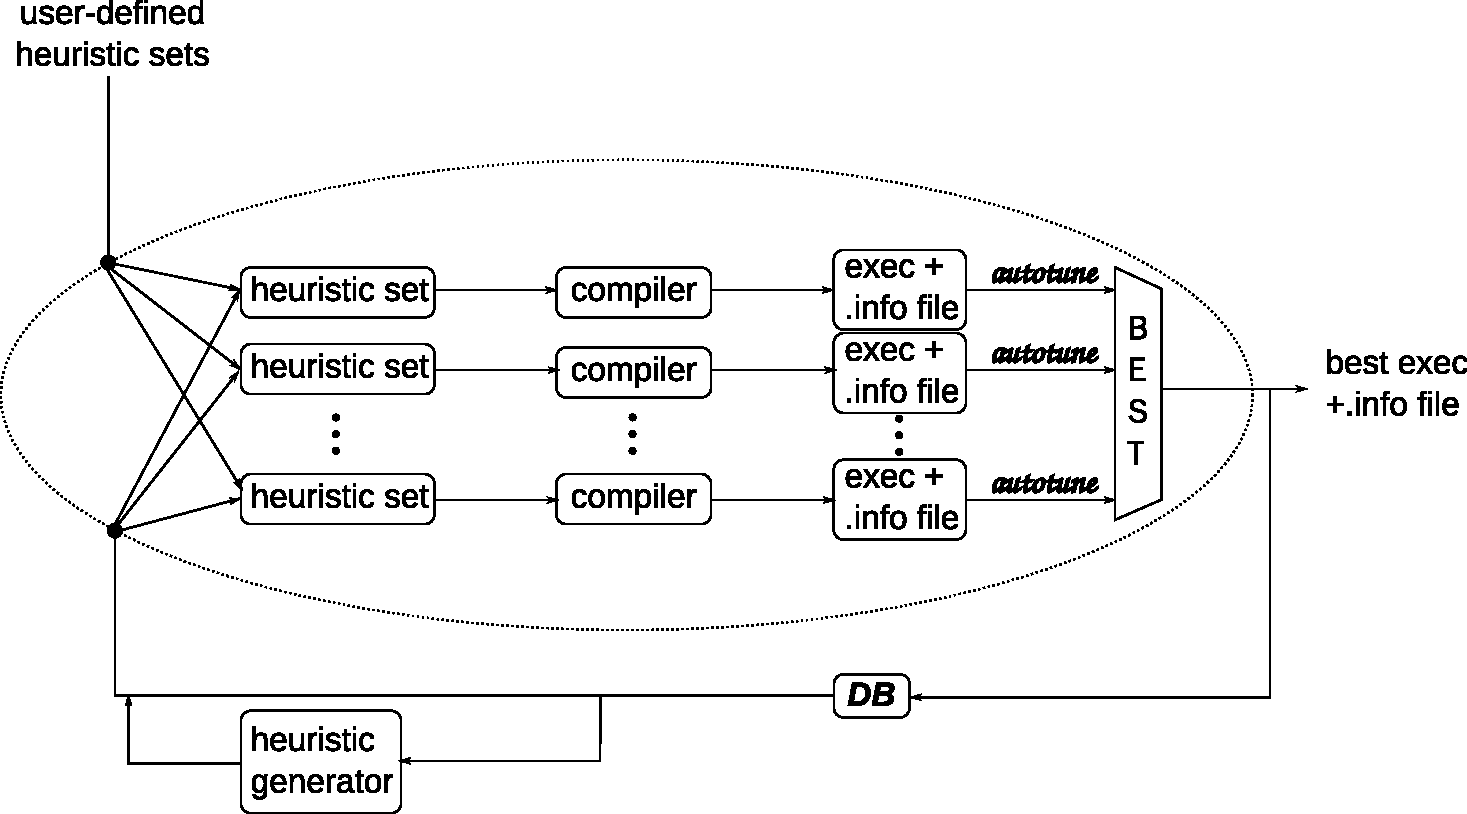
\includegraphics[width=\textwidth]{heurArchitecture}

The compilation scripts take as their input a XML file structured like this:
\begin{verbatim}
<heuristics>
  <set>
    <heuristic name="thisHeuristic" formula="(foo+bar) / foobar" />
    <heuristic name="thatHeuristic" formula="if var1+var2 &lt; 3 then 5 else 7" />
  </set>
  <set>
    <heuristic name="thisHeuristic" formula="5 * a + 8" />
  </set>
  <set>
    <heuristic name="otherHeuristic" formula="21 - a + 8*b" />
  </set>  
</heuristics>
\end{verbatim}

The file includes a bunch of heuristics sets.
Every set will be used as the input for a  different instance of the compiler, generating different executable files. All the executable files will be autotuned, and the best one will be chosen.
Then, the data about the results obtained by the various files are stored in the database (\texttt{knowledge.db} in the \texttt{$\sim$/tunerout} directory).

The sets can be incomplete, not including all the required heuristics.
The missing heuristics will be automatically taken from the database or, with a given probability, from the heuristic generator. If the database is empty and the heuristic generator did not generate any new heuristic, the system will fall back to using the default heuristic specified by the programmer inside the compiler itself.

\section{Classes in petabricks}
Three C++ classes implemente this framework into Petabricks

\subsection{Heuristic}
Represents a heuristics in the compiler.

The public interface includes:
\begin{description}
 \item[formula()] return the formula representing the heuristic.
 \item[eval(ValueMap featureValues)] return the evaluation of the heuristic. ValueMap is a map name-value of the values that will be substituted to each of the features (variables) that appear in the formula. The evaluation is the number obtained by substituting the features with the values in the given map.
\end{description}

\subsection{HeuristicManager}
The heuristic manager is the main point of interaction for the compiler writer with the long term learning system.

It provides the following methods:
\begin{description}
 \item [instance()] this static method returns the singleton instance of the HeuristicManager. It can be invoked from everywhere inside the compiler itself.
 \item [getHeuristic(string name)] return a heuristic given its name. The name should be chosen to be different for heuristics having different meaning. The heuristic is taken, in order, from the input file specified on the command line, from the database (the best heuristic is taken) or from the default
 \item [registerDefault(string name, string formula)] register \texttt{formula} as the default heuristic named \texttt{name}. NB: before using \texttt{getHeuristic} on any name, a default heuristic for that name should always be registered, so that the compiler can always work properly, even without an input file and with an empty database.
\end{description}


\subsection{DBManager}
Is responsible for managing the database. It should never be used directly.

\section{Scripts}
The learning part is performed by a series of python scripts

\subsection{learningcompiler.py}
Contains all the logic dealing with the long term learning of heuristics.
It can also be used to compile a single program using a given set of heuristics.

To do this, run:

\texttt{learningcompiler.py <heuristicsFile> <program.pbcc>}

\subsection{formula.py, maximaparser.py}
They contain the python representation of formulas and the parser.

\subsection{smoketest.py, pbbenchmark.py}
The default behaviour of the scripts is unchanged.

Invoking the scripts with the \texttt{--learning} parameter activates the learning of new heuristics, starting from those already present in the database.

Invoking the scripts with the \texttt{--heuristics=<filename>} implies \texttt{--learning}, but uses first the heuristics taken from the input file.



\end{document}